\chapter{Embodiment Design}
The next phase in the design methodology is embodiment design. This phase, as defined by Pahl and Beitz \cite{Pahl07t}, involves starting with the fundamental solution or concept for a technical product and then advancing the design in alignment with technical and economic criteria, taking into account further information. The ultimate objective is to reach a stage where the subsequent detailed design can smoothly progress into the production phase.
Figure \ref{fig:embodiment_design} shows the steps involved in this phase.

\begin{figure}
    \centering
    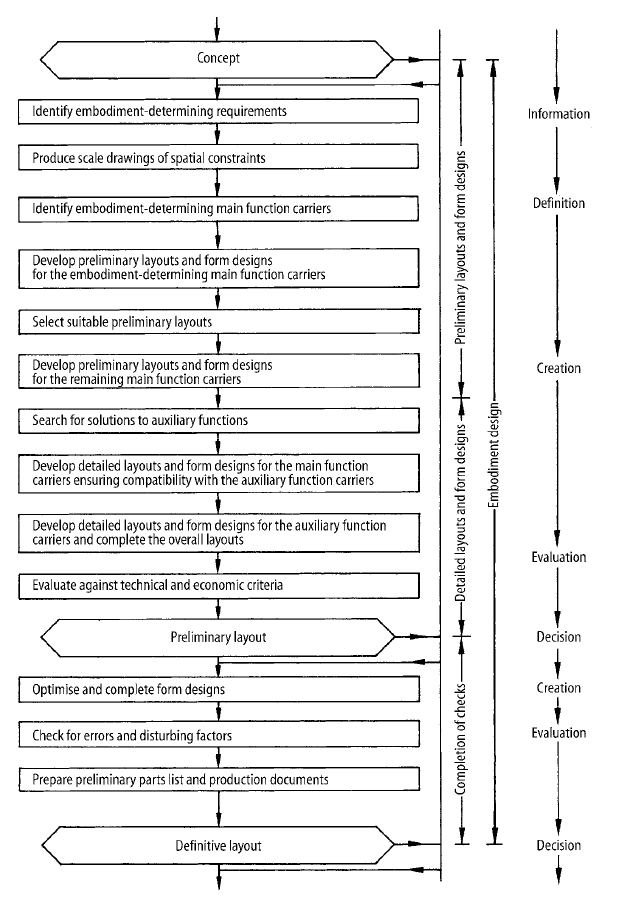
\includegraphics[width=0.92\linewidth]{texs/Part1/chapter4/image/embodiment.png}
    \caption{Steps in Embodiment Design \cite{Pahl07u}}
    \label{fig:embodiment_design}
\end{figure}

\section{Basic Rules of Embodiment Design}
When it comes to product design, there are some basic rules that must be followed. As defined by Pahl and Beitz \cite{Pahl07v}, they include clarity, simplicity, and safety. Neglecting these rules can potentially result in issues and accidents. Subsequent sections will provide a comprehensive exploration of these guidelines.

\subsection{Clarity}
Clarity, as described by Pahl and Beitz \cite{Pahl07w}, entails establishing clear and unambiguous connections within a design. This involves ensuring straightforward relationships between subfunctions, inputs, and outputs to prevent any confusion or misinterpretation. It also extends to the selection of a working principle, where designers should choose principles that clarify cause-and-effect dynamics, align with the product's purpose, and optimize its layout by eliminating unnecessary complexity.

Additionally, clarity applies to the broader design structure, whether it involves multiple working principles or component combinations. It mandates that the design facilitates the orderly flow of energy, materials, and signals, preventing adverse effects like excessive forces or wear. This commitment to clarity ultimately enhances the product's reliability and durability.

\subsection{Simplicity}
Simplicity \cite{Pahl07x} in design is epitomized by an uncomplicated and easily comprehensible approach, often achievable by using fewer components. Such simplicity can lead to cost savings, reduced wear and tear, and minimized maintenance requirements. Nonetheless, it's crucial to strike a balance, as certain functions inherently demand a minimum number of components.

Designers should, therefore, strive for a minimalist approach by employing the fewest components possible while maintaining straightforward shapes, as this promotes efficiency and practicality in the design process. The choice between numerous components with simple shapes, albeit potentially increasing production effort, and a single, more affordable cast component should be made while considering the specific problem and constraints.

\subsection{Safety}
Safety \cite{Pahl07y} considerations are crucial in ensuring both the effective performance of technical functions and the protection of people and the environment. Designers rely on a safety methodology outlined in the German industry standard DIN 31 000, which encompasses three levels: direct safety, indirect safety, and warnings. In general, designers should prioritize direct safety measures, seeking solutions that inherently eliminate potential dangers. Only when this is not feasible should they resort to indirect safety measures, involving the construction of specialized protective systems.

Warnings, which serve to highlight dangers and hazard zones, are best utilized in conjunction with direct and indirect safety measures, clarifying specific risks. As designers address technical challenges, they encounter various constraints, not all of which can be simultaneously overcome. However, their objective remains to develop solutions that come as close as possible to meeting all requirements. It's important to note that exceptionally high safety demands can complicate design, potentially diminishing clarity and economic viability, and even leading to project abandonment in some cases.

\section{Guideline of Embodiment Design}
In addition the the basic rules of embodiment design, Pahl and Beitz \cite{Pahl07z} also stress the importance of following a set of design guidelines to help designers meet the specific requirements and constraints. For this project, the following design guidelines are considered:

\begin{itemize}
    \item Design for production
    \item Design for ergonomics
\end{itemize}

\subsection{Design for Production}
Design for production \cite{Pahl07aa} is a design guideline that emphasizes the importance of considering the production process during the design phase. This approach enables designers to optimize the production cost and times while ensuring the product's functionality and quality. By following the basic rules of clarity and simplicity, designers are already on the right track to achieving this goal.

\subsubsection{Appropriate Overall Layout Design}
Overall layout design, derived from the function structure, influences product division into assemblies and components, including sourcing decisions (in-house, bought-out, standard parts), production procedures, dimensions, batch sizes, joining methods, and quality control.

The layout can lead to differential, integral, composite, or building-block construction methods. Differential Construction involves breaking down components into easily produced parts, facilitating adaptability, increased component batch sizes, and easier quality assurance. However, it demands greater machining and assembly costs and may have functional limitations due to joints.

Integral Construction combines multiple parts into a single component, reducing costs due to integration but can be complex and sensitive to market conditions. Composite Construction involves connecting different parts requiring further work, applying multiple joining methods or using various materials for optimal property utilization.

Building Block Construction results from splitting components so that the parts or assemblies can be used in other products or variants, offering flexibility and cost savings. These construction methods offer specific advantages and disadvantages, depending on the context and design requirements.

\subsubsection{Appropriate Form Design of Components}
During component form design, designers significantly impact production costs, times, and product quality by choosing shapes, dimensions, surface finishes, tolerances, and fits. These choices influence production procedures, machine types, in-house vs. bought-out components, materials, and quality control procedures.

Conversely, production facilities influence design features, which may include dimension limitations necessitating component division or the acquisition of bought-out components. Many guidelines exist for appropriate component form design, and tolerances are crucial.
Figure \ref{fig:guideline} shows the design guidelines for designing components specifically for 3D printing.

\begin{figure}
    \centering
    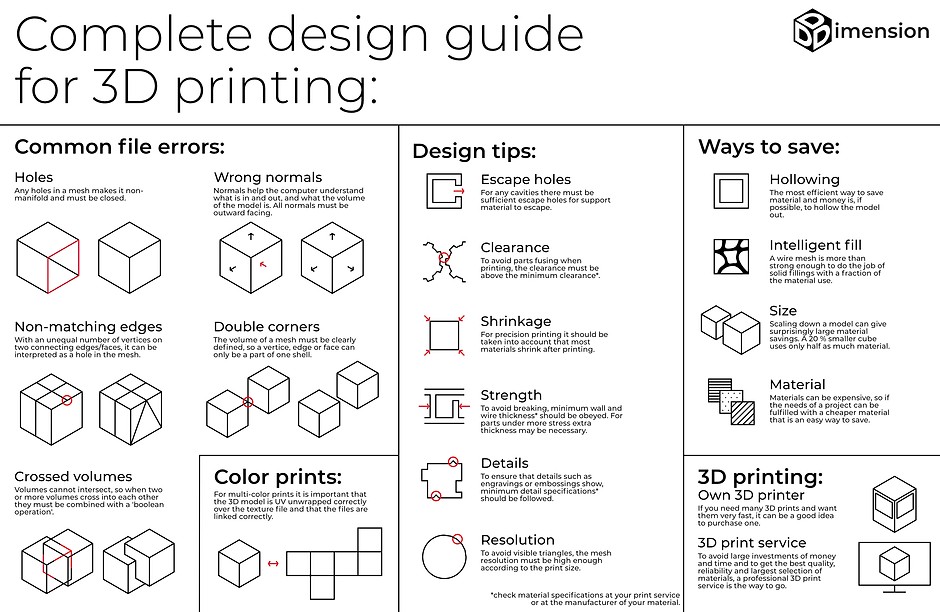
\includegraphics[width=0.92\linewidth]{texs/Part1/chapter4/image/guidelines.png}
    \caption{Design guidelines for 3D printing \cite{DDDimension_22}}
    \label{fig:guideline}
\end{figure}

\subsection{Design for Ergonomics}
Ergonomics \cite{Pahl07ab} is vital in designing technical products, aiming to align them with human characteristics, needs, and interfaces. It covers a broad range of items, including everyday household products and human-machine interfaces. Recent focus has shifted to user-friendly interfaces and ergonomic workplace assessment tools.

Ergonomic design considers various factors, starting with biomechanics, which addresses how body postures and movements interact with product design. Physiological aspects, such as muscle action, circulation, and temperature regulation, are crucial. Sensory factors like light and noise must also be taken into account. Psychological aspects guide design to minimize cognitive load and enhance user-friendliness.

Ergonomics extends to active and passive user involvement. Active involvement necessitates careful planning, assessing if human interaction is necessary and effective. Passive involvement addresses how users are affected by products, considering factors like energy flows, vibrations, light, climate, and noise.

Identifying ergonomic requirements can follow two approaches. The object-based approach is used when designing predefined systems or products, employing checklists tailored to specific items. The effect-based approach applies to new situations, analyzing the effects of energy, material, and signal flows, ensuring they meet ergonomic requirements. Both aim to prioritize user comfort, safety, and efficiency while minimizing discomfort and errors.



% https://www.ddd-imension.com/en/post/complete-design-guide-for-3d-printing

% https://www.hubs.com/get/3d-printing-design-rules/

\section{Preliminary Design}
In this section, we will explore the preliminary design of the device. The preliminary design is detailed 3D model of the device that will be used to evaluate the design and determine its feasibility. The preliminary design will be based on the selected solution from the previous phase. Along with the model, the production cost will be also presented in this section. For a more detailed calculation of the production cost, please refer to Appendix \ref{appendix:production_cost}.


\subsection{Preliminary Design Variant 2}
This section delves into a detailed exploration of Solution Variant 2. Figure \ref{fig:preliminary_design_variant_2} shows the preliminary design variant 2 and different views and body measurement are shown in Figure \ref{fig:variant2_views}. The main attraction of this design is the emphasis on ergonomic form and user-friendly features. The device incorporates a sleek and aesthetically pleasing design with rounded edges and a lightweight build, making it easily portable and comfortable to hold for extended periods. With a thickness of 46 mm (Figure \ref{fig:variant2_right_view}), the device strikes a balance between being slim and accommodating the necessary components for optimal functionality .

\begin{figure}[h!]
    \centering
    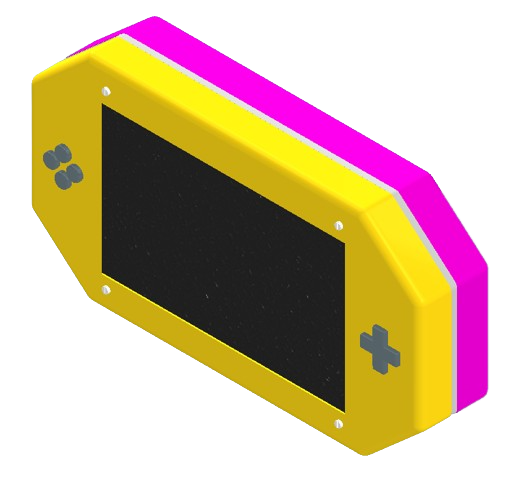
\includegraphics[height=5 cm]{texs/Part1/chapter4/image/v21.png}
    \caption{Preliminary design variant 2}
    \label{fig:preliminary_design_variant_2}
\end{figure}

\begin{figure}[h!]
    \centering
    \begin{subfigure}[c]{0.65\textwidth}
        \begin{minipage}{\textwidth}
            \centering
            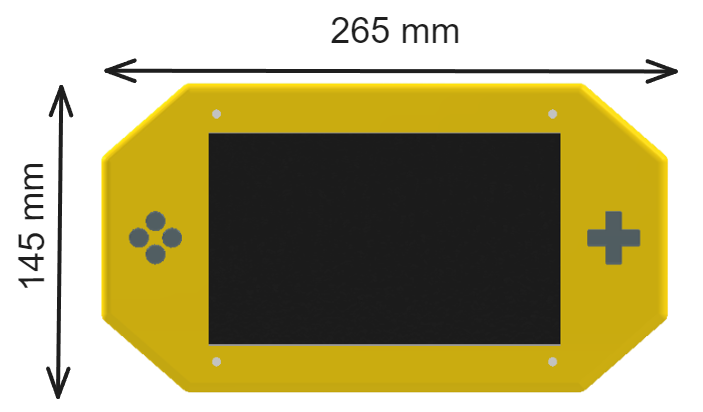
\includegraphics[height=4 cm]{texs/Part1/chapter4/image/v22.png}
        \end{minipage}
        \caption{Front View}
        \label{fig:variant2_front_view}
    \end{subfigure}
    % \hfill
    \begin{subfigure}[c]{0.25\textwidth}
        \begin{minipage}{\textwidth}
            \centering
            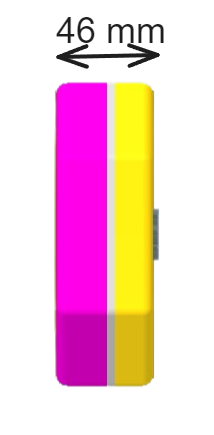
\includegraphics[height=4 cm]{texs/Part1/chapter4/image/v23.png}
        \end{minipage}
        \caption{Right View}
        \label{fig:variant2_right_view}
    \end{subfigure}
    \caption{Views of preliminary design variant 2}
    \label{fig:variant2_views}
\end{figure}

\begin{figure}[h!]
    \centering
    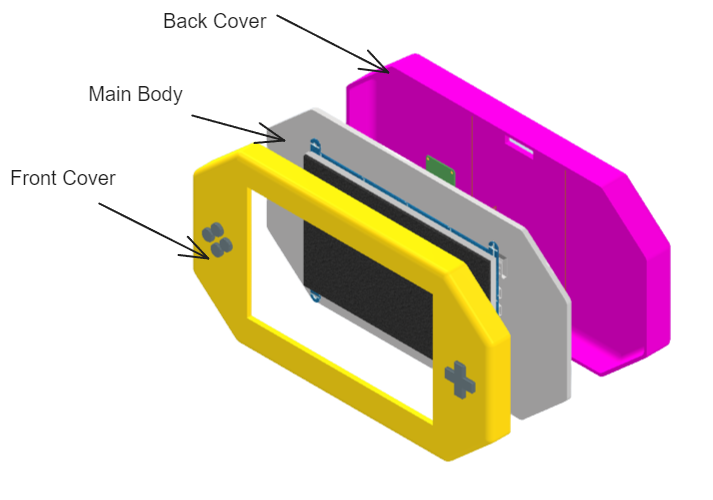
\includegraphics[width=0.5\linewidth]{texs/Part1/chapter4/image/v24.png}
    \caption{Body Components of preliminary design variant 2}
    \label{fig:variant2_body_components}
\end{figure}

\begin{figure}[h!]
    \centering
    \begin{subfigure}[c]{0.47\textwidth}
        \begin{minipage}{\textwidth}
            \centering
            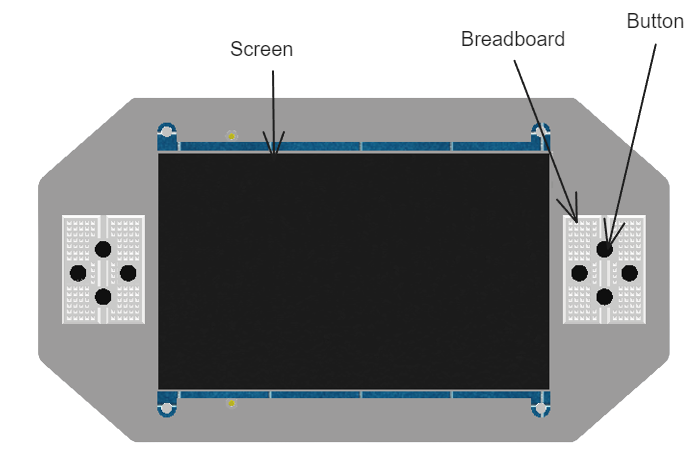
\includegraphics[height=4 cm]{texs/Part1/chapter4/image/v25.png}
        \end{minipage}
        \caption{Front View}
        \label{fig:variant2_front_view_main}
    \end{subfigure}
    % \hfill
    \begin{subfigure}[c]{0.47\textwidth}
        \begin{minipage}{\textwidth}
            \centering
            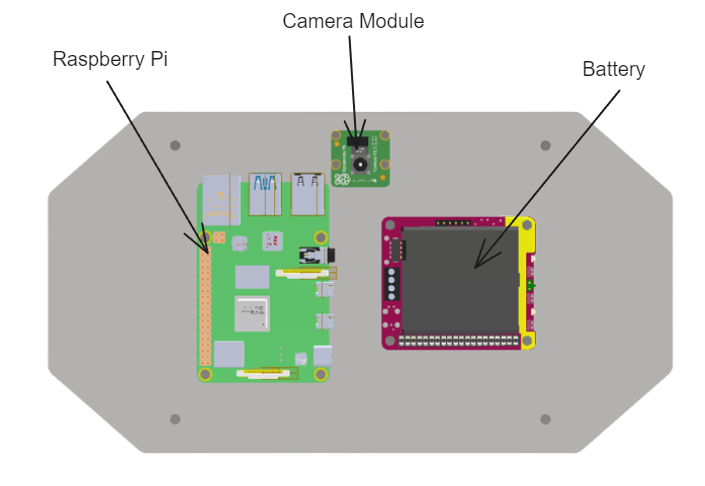
\includegraphics[height=4 cm]{texs/Part1/chapter4/image/v26.png}
        \end{minipage}
        \caption{Back View}
        \label{fig:variant2_back_view_main}
    \end{subfigure}
    \caption{Placement of inner components}
    \label{fig:variant2_inner_components}
\end{figure}

The physical design of Solution Variant 2 follows a carefully crafted sandwich-like structure, consisting of a main body, top cover, and back cover (Figure \ref{fig:variant2_body_components}). This design choice not only ensures the protection of the internal components but also facilitates ease of assembly and maintenance. The main body serves as the central hub, housing all the essential electronics and functional elements, while the top and back covers act as protective layers, safeguarding the delicate components from potential damage due to external impacts.


A key consideration in the design is the arrangement of the inner components within the device. Following a tablet-like configuration, the main LCD is thoughtfully positioned on the front side of the main body, providing users with a clear and interactive interface (Figure \ref{fig:variant2_front_view_main}). Meanwhile, the camera, Raspberry Pi, and battery are strategically placed on the back side of the body (Figure \ref{fig:variant2_back_view_main}), optimizing the distribution of weight and ensuring a well-balanced user experience. This arrangement also enhances the device's overall usability and convenience, making it suitable for a wide range of applications.


\begin{figure}[ht!]
    \centering
    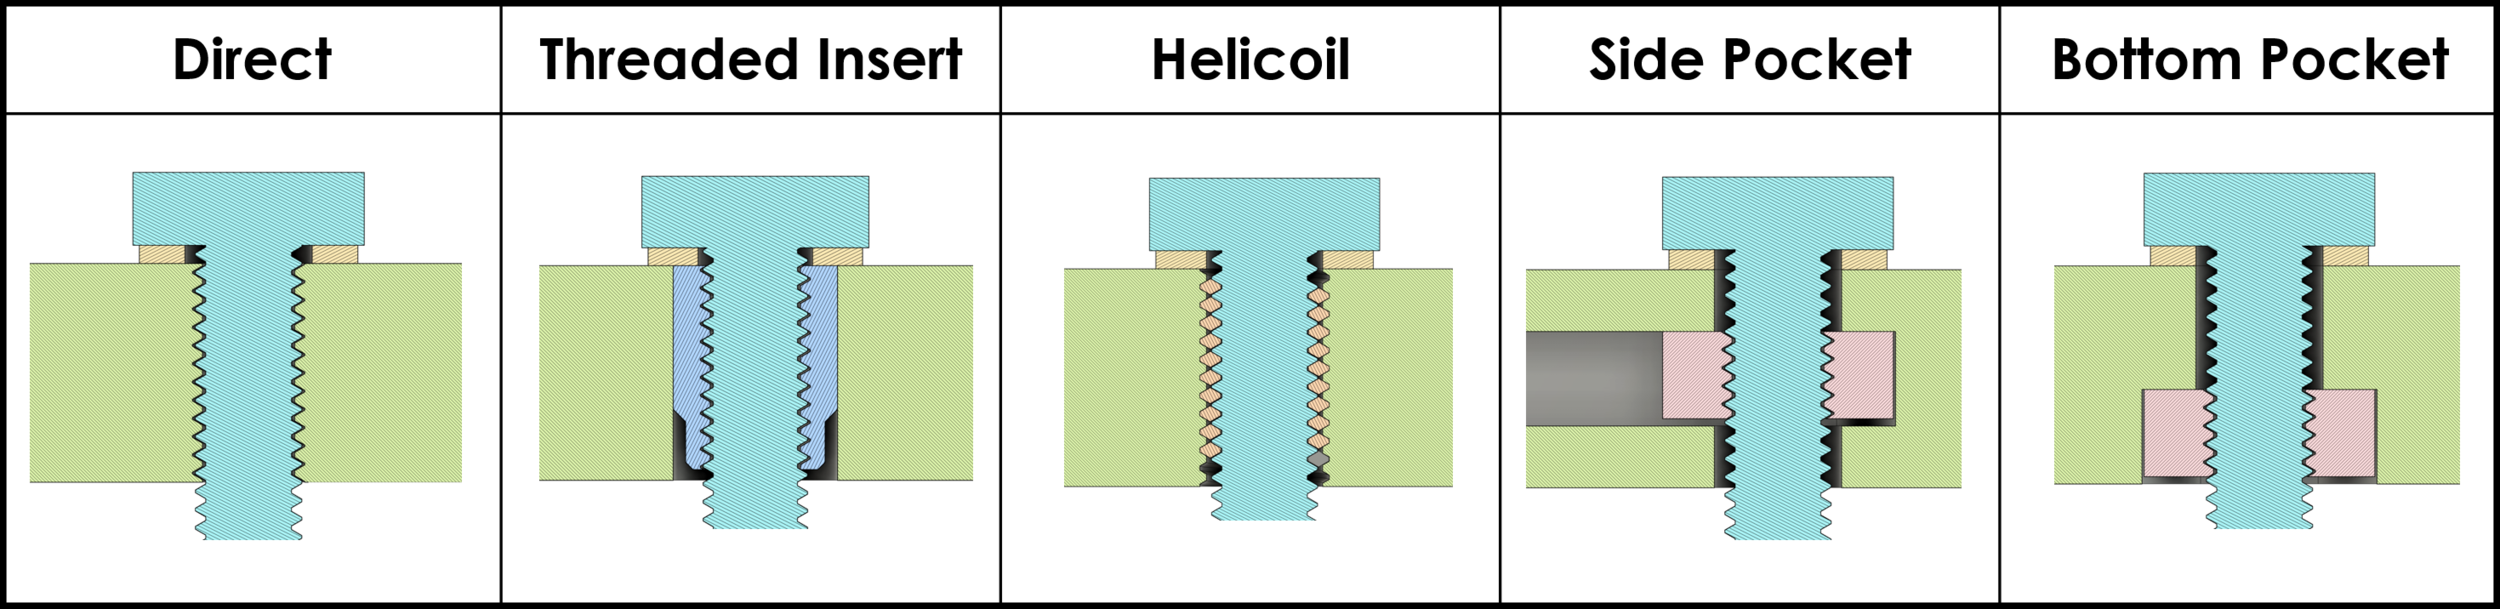
\includegraphics[width=\linewidth]{texs/Part1/chapter4/image/insert.png}
    \caption{Methods to secure components \cite{Hermann20}}
    \label{fig:insert}
\end{figure}


Ensuring the secure attachment of components to the main body is of paramount importance in the design process. Various methods for component fastening are considered, including direct attachment, threaded inserts, helicoils, side pockets, and bottom pockets as shown in Figure \ref{fig:insert}.

The simplest approach is direct attachment, where threads are designed into the 3D printed part to allow components to be screwed in. For more robust connections, threaded inserts can be used by designing holes in the 3D printed part and installing the inserts appropriately.

Helicoils offer durable threaded holes by inserting coil-shaped inserts into designed holes. Side pockets and bottom pockets involve creating cavities or slots in the 3D printed part to securely hold components. Each method offers its own set of advantages and challenges, and after careful evaluation, the variant opts for the use of threaded inserts due to their simplicity and robustness.

The battery, being a critical component within the device, requires special attention to prevent any undesirable movement or instability. Figure \ref{fig:variant2_battery_cover} shows the battery cover which will be attached to the main body, while Figure \ref{fig:variant2_battery_placement} shows the method of securing the battery to the main body.


To address this concern, an effective method for securing the battery firmly in place is implemented by utilizing a battery cover. The battery cover is then securely attached using screws and standoffs, ensuring that the battery remains in its designated position even during vigorous handling or movement.

\begin{figure}[h!]
    \centering
    \begin{subfigure}[c]{\textwidth}
        \begin{minipage}{\textwidth}
            \centering
            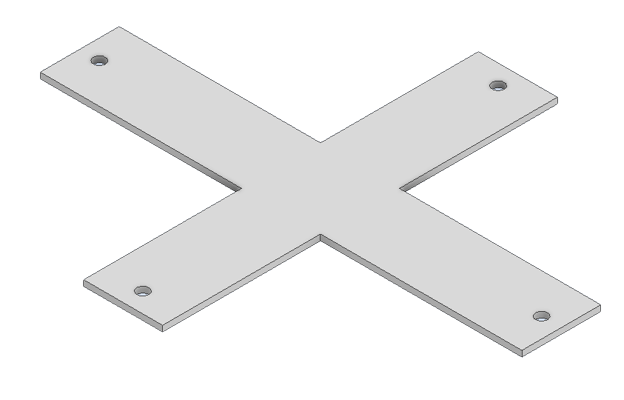
\includegraphics[height=4 cm]{texs/Part1/chapter4/image/v27.png}
        \end{minipage}
        \caption{Battery Cover}
        \label{fig:variant2_battery_cover}
    \end{subfigure}
    % \hfill
    \begin{subfigure}[c]{\textwidth}
        \begin{minipage}{\textwidth}
            \centering
            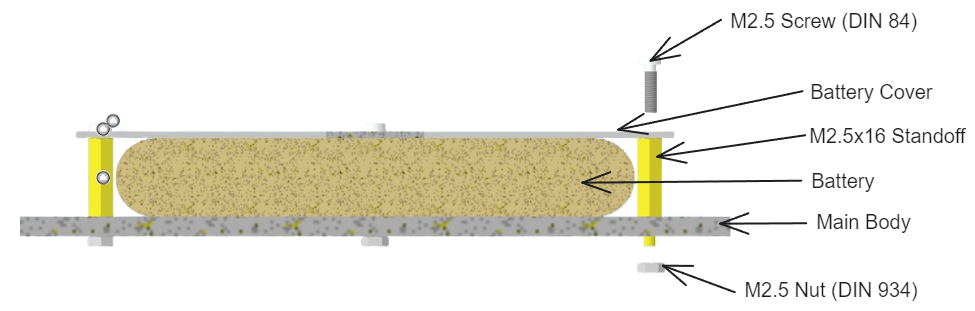
\includegraphics[height=3 cm]{texs/Part1/chapter4/image/v28.png}
        \end{minipage}
        \caption{Placement of components}
        \label{fig:variant2_battery_placement}
    \end{subfigure}
    \caption{Methods to secure the battery}
    \label{fig:variant2_battery}
\end{figure}


Solution Variant 2 will employ a hybrid input method, combining both touch screen and physical buttons. The touch screen will be oriented in landscape mode, while the buttons will be positioned on either side of the screen (Figure \ref{fig:variant2_front_view}). To enable the integration of the touch screen, HDMI and USB connections will be established between the touch screen and the Raspberry Pi \cite{Sunfounder}. Additionally, to facilitate the functionality of the physical buttons, they will be connected to the Raspberry Pi using its GPIO (General Purpose Input/Output) pins \cite{Soren21}.

\begin{figure}[ht!]
    \centering
    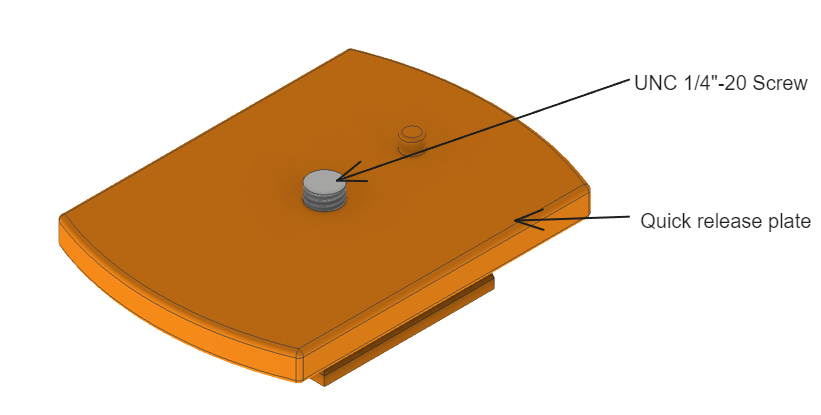
\includegraphics[height=5 cm]{texs/Part1/chapter4/image/v29.png}
    \caption{Quick release plate}
    \label{fig:variant2_quick_release_plate}
\end{figure}

In Figure \ref{fig:variant2_quick_release_plate}, we can observe the quick release plate designed to be affixed to the tripod stand. For enhanced stability during usage, Solution Variant 2 can utilize the quick release plate which can be conveniently mounted on a tripod stand.

\subsubsection{Cost Calculation}
In this section, we will perform a cost analysis for producing Solution Variant 2. It is essential to emphasize that the cost calculation for the 3D printed parts solely considers the material cost and the estimated energy consumption during the printing process. Other expenses, such as the cost of the 3D printer itself, labor, and maintenance, are not factored into the calculation. Additionally, for better comparability with other variants, the costs of the Raspberry Pi, camera module, touch screen, and battery will not be included in the calculation. The formula used to calculate the cost of the 3D printed parts is as follows:

\dots


\subsection{Preliminary Design Variant 3}


Figure \ref{} presents an insightful glimpse into the conceptualization of preliminary design variant 3. Much akin to variant 2, the arrangement of components exhibits striking resemblances, wherein the screen adorns the frontal expanse, while the camera, Raspberry Pi, and battery find their abode at the rear. However, a notable deviation takes form in variant 3, as the screen's orientation transforms into portrait mode, and a fascinating alteration emerges in the positioning of the computational unit and battery—they are now artfully stacked atop one another.

The chassis structure, reminiscent of variant 2, boasts a harmonious triad of the main body, top cover, and back cover. Manifesting as the nucleus of the device, the main body houses an orchestration of vital electronics and functional intricacies. Meanwhile, the top and back covers diligently assume the mantle of guardians, cocooning the device's delicate components from potential harm inflicted by external forces.

A compelling divergence emerges in the form of a tactile innovation—a subtle yet meaningful bump graces the back cover. This augmentation is a deliberate endeavor to enhance the device's ergonomics, tailored to seamlessly nestle within the contours of the user's palm. The result is an intuitively comfortable grip that heightens user engagement and prolongs usability.

Distinctive alteration in battery placement marks yet another departure from variant 2's blueprint. Abandoning the concept of a dedicated battery cover, variant 3 strategically carves a snug slot within the back cover's canvas. This niche is bespoke to accommodate the battery, eliminating any possibility of unwanted shifts during device operation. Such ingenuity streamlines the process of battery replacement, ushering in an era of swift and effortless renewals.

The input methodology undergoes a streamlining, harnessing the prowess of the touch screen as the singular interface. This approach offers a streamlined user experience, unfettered by physical buttons, and seamlessly marries the screen with user interaction. A comprehensive elucidation of the touch screen's connection to the Raspberry Pi is expounded upon in a prior section, ensuring a symphony of function and compatibility.

The harmonious integration of the chassis with the tripod stand unfolds through a direct union. The tripod stand's mounting point affixes itself with grace to the underbelly of the main body. Meticulous scrutiny of the quick release plate's design yields an intriguing revelation—the focal point of attachment between the plate and the tripod stand rests upon the trapezoidal contour. Ingeniously, this prism becomes an organic extension of the main body, seamlessly embracing the tripod stand. The net result is an effortlessly achieved amalgamation, ushering the device into a realm of enhanced stability and versatile usage scenarios.

\subsubsection{Cost Calculation}

\subsection{Preliminary Design Variant 6}

The unveiling of Figure \ref{} offers an illuminating exposition of the preliminary design variant 6. This iteration boldly forges a distinctive path, setting itself apart by orchestrating its internal components in a configuration reminiscent of the point-of-service (POS) system. A prominent departure from previous renditions, this design choice strategically aligns the screen at an angle, fostering effortless user interaction. This ingenious placement optimizes screen visibility, facilitating seamless engagement for the user. Furthermore, a striking juxtaposition of the battery and Raspberry Pi unfolds on the device's frontal landscape, one atop the other. To ensure structural integrity, the attachment of these components is meticulously executed through the use of screws and threaded inserts, as previously elucidated.

Manifesting as an embodiment of thoughtful design, this variant is encapsulated by a bowl-like chassis structure. A symbiotic synergy of the main body, serving as the guardian of internal components, and a top cover, adorning the device with an added layer of protection, defines the architectural essence of this design.

The realm of user experience is skillfully curated through the seamless integration of a handle grip nestled beneath the device. This strategic implementation empowers users with a comfortable grip, ensuring prolonged usage remains effortless and enjoyable. Alternatively, this ingenious handle grip serves as an anchor point for attaching the quick release plate—a gateway to mounting the device on a tripod stand. This multifaceted utility imbues the device with enhanced versatility, seamlessly transitioning from handheld to mounted scenarios.

A familiar melody resonates in the input methodology and battery placement of this variant, akin to the orchestrations observed in variant 3. The touch screen takes center stage as the primary input mechanism, offering an intuitive and streamlined interaction experience. Similarly, the battery finds its abode within a specially crafted slot on the back cover, securely fastened in place by the steadfast embrace of screws and threaded inserts. This ergonomic battery placement facilitates easy removal and replacement, underscoring the design's practicality and user-centric ethos.

\subsubsection{Cost Calculation}


\subsection{Preliminary Design Variant 7}

The unveiling of Figure \ref{} offers a captivating insight into the preliminary design variant 7, a configuration ingeniously influenced by the handheld PC paradigm. In this rendition, the raspberry pi stakes its claim on the rear side of the screen, creating an integrated and compact composition. Concurrently, the battery aligns itself in symphony, gracefully nestling alongside the screen in a harmonious juxtaposition.

The design ethos extends to the chassis structure, which draws inspiration from the bowl-like form of variant 6. This architectural continuity ensures a cohesive aesthetic while enabling seamless integration of functional components.

In the realm of user handling, a clever innovation akin to variant 3 is introduced, albeit with a distinctive twist. A strategically positioned bump adorns the side of the body, offering an ergonomic touch that resonates with the user. Remarkably, this bump also serves as a sanctum for the battery, providing a secure and discreet enclosure within the device's contours. Notably, in variant 7, the battery finds its dwelling as a permanent fixture within the device, fortifying its structural stability.

The control mechanisms of this variant mirror those observed in variant 2, embracing a synthesis of tactile and touch interfaces. The touch screen assumes the mantle of the primary input mechanism, engaging users in an intuitive and seamless dialogue with the device. Complementing this touch-driven interaction, physical buttons find their abode along the device's side, imbuing the design with a secondary input avenue.

In a fitting culmination, akin to the design philosophy of variant 3, the integration of the device with a tripod stand materializes through a direct symbiosis. A trapezoidal prism, an architectural marvel in its own right, becomes an extension of the device's body, facilitating a straightforward alliance with the tripod stand. This elegant integration underscores the design's commitment to stability and adaptability, transforming the device into a versatile tool suited for a spectrum of scenarios.


\subsubsection{Cost Calculation}

\section{Evaluation of Preliminary Design Variants}
VDI 2225

\subsection{Evaluation Criteria}

The technical evaluation criteria are primarily derived from the list of requirements but can also be established from general conditions. The property dimensions can be captured through specific metrics as well as qualitative statements. When establishing the evaluation criteria, it must be noted that the individual goals to be evaluated are largely independent from each other. The identified criteria must be formulated positively, as this enables better alignment with the corresponding value concepts.37 The following evaluation criteria are used for the technical assessment of the various variants:

\textbf{Ergonomics:} The ergonomics of the variants are evaluated based on the following criteria: \textit{handling, weight, and dimensions}. The handling is assessed based on the ease of use and the intuitive operation of the variants. The weight is evaluated based on the weight of the variants and the weight distribution. The dimensions are assessed based on the size of the variants and the size of the individual components.

\textbf{Weight Distribution:} The weight distribution is evaluated based on the weight distribution of the variants and the weight distribution of the individual components. The value for weight distribution is retrieved from Computer-Aided Design (CAD) models through detailed analysis of the device's structural layout and component placement.

\textbf{Device Weight:} Device weight evaluates the overall heaviness of the equipment. A lighter device is generally easier to handle and transport, reducing user fatigue and enabling greater mobility while maintaining performance and durability. The value for device weight is calculated from Computer-Aided Design (CAD) models by summing the individual weights of all components, materials, and structural elements that constitute the device.

\textbf{Device Size:} The size criterion considers the physical dimensions of the device, assessing its compactness and portability. An optimal device size allows for convenient storage, transportation, and operation in various environments without compromising functionality. The evaluation of device size involves measuring key dimensions such as length, width, height, and any protrusions or extensions.

\textbf{Ease of Assembly:} This criterion focuses on the simplicity and efficiency of assembling and disassembling the device. A design that enables quick and hassle-free assembly and disassembly not only saves time but also enhances user convenience and reduces the risk of errors. Evaluation is conducted by assessing the number of components involved in the assembly and disassembly processes. A lower count of components often indicates a simpler and more user-friendly design. Additionally, the type and quantity of fasteners, such as screws or connectors, required for assembly are taken into account. A reduced reliance on intricate fastening mechanisms contributes to smoother handling and maintenance. By quantifying these factors, designers can gauge the ease of assembly and disassembly, enabling them to refine the design to optimize user-friendliness and operational efficiency.

\textbf{Swappable Parts:} Swappable parts assess the ease with which components or parts of the device can be interchanged or replaced. A design that facilitates swappable parts enhances flexibility, maintenance, and adaptability to different tasks or conditions. Swappable parts promote component modularity, enabling efficient repairs and upgrades. The evaluation of swappable parts is based on the number of interchangeable components and their compatibility across the device. A higher number of swappable parts indicates a design that encourages versatility and minimizes downtime during maintenance or repairs. This modularity simplifies troubleshooting and allows users to adapt the device to evolving needs or specialized requirements. By quantifying the availability of swappable parts, designers can ensure a design that empowers users to swiftly and effectively manage the device's functionality, enhancing its overall usability and lifespan.

\textbf{Durability to External Factors:} Durability to external factors evaluates how well the device can withstand exposure to various environmental conditions, such as humidity, temperature fluctuations, dust, and impacts. A high level of durability ensures a longer lifespan and consistent performance under diverse circumstances. The assessment of durability is measured by estimating the number of openings in the device. More openings can lead to greater exposure of inner components, potentially making them susceptible to external elements. Therefore, a design with fewer openings is considered more resilient, as it reduces the likelihood of environmental factors affecting critical components. By quantifying the number of openings and assessing their placement, designers can enhance the device's ability to endure harsh conditions and maintain reliable functionality over time, ultimately extending its operational life and user satisfaction.



